% TikZ diagram for black-box safety validation problem formulation.
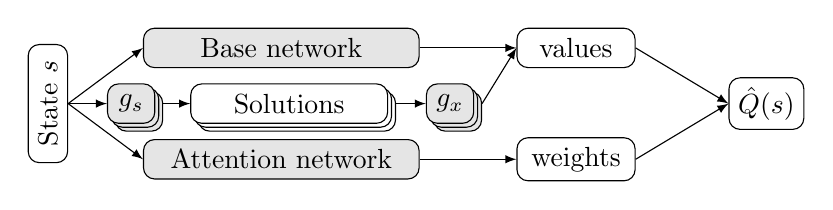
\begin{tikzpicture}
    \tikzstyle{every node}=[font=\normalsize, align=center]
    \tikzset{
        n/.style={draw, rounded corners, minimum height=0.5cm, minimum width = 1.5cm},
        n2/.style={n, minimum width=3.5cm},
        n4/.style={n, minimum width=2.5cm},
        n3/.style={n, minimum width=0.6cm}
        }
    
    %state 
    \node (state) [n, rotate=90] { State $s$};
    
    %base network
    \node (base) [n2, fill=black!10, above right of=state, anchor=west, xshift=0.5cm] {Base network};
    
     %State Transforms
    \node (stback1) [n3, fill=black!10, right of=state, anchor=west, xshift=-0.15cm, yshift=-0.1cm] {};
    \node (stback2) [n3, fill=black!10, right of=state, anchor=west, xshift=-0.2cm, yshift=-0.05cm] {};
    \node (st) [n3, fill=black!10, right of=state, anchor=west, xshift = -0.25cm] {$g_s$};
    
    %Solutions
    \node (solutionsback1) [n4, right of=st, xshift=-.15cm, yshift=-0.1cm, anchor=west] {};
    \node (solutionsback2) [n4, fill=white, right of=st, xshift=-0.2cm, yshift=-0.05cm, anchor=west] {};
    \node (solutions) [n4, fill=white, right of=st, anchor=west, xshift = -0.25cm] {Solutions};
    
    %Action Transforms
    \node (atback1) [n3, fill=black!10, right of=solutions, anchor=east, xshift=1.45cm, yshift=-0.1cm] {};
    \node (atback2) [n3, fill=black!10, right of=solutions, anchor=east, xshift=1.4cm, yshift=-0.05cm] {};
    \node (at) [n3, fill=black!10, right of=solutions, anchor=east, xshift=1.35cm] {$g_x$};
    
    %weights
    \node (attn) [n2, fill=black!10, below right of=state, anchor=west, xshift=0.5cm] {Attention network};
    

    \node (values) [n, right of=base, anchor=east, xshift=3.5cm] {values};
    
     \node (weights) [n, right of=attn, anchor=east, xshift=3.5cm] {weights};
     
     \node (pfail) [n, minimum width = 0.5cm, right of=at, anchor=east, xshift=3.5cm] {$\hat{Q}(s)$};
    

    \draw[-latex] (state.south) -- (base.west);
    \draw[-latex] (state.south) -- (st.west);
    \draw[-latex] (st.east) + (0.1cm, 0cm) -- (solutions.west);
    \draw[-latex] (solutions.east) + (0.1cm, 0cm) -- (at.west);
    \draw[-latex] (state.south) -- (attn.west);
    
    \draw[-latex] (base.east) -- (values.west);
    \draw[-latex] (at.east) + (0.1cm, 0cm) -- (values.west);
    \draw[-latex] (attn.east) -- (weights.west);
    
    \draw[-latex] (weights.east) -- (pfail.west);
    \draw[-latex] (values.east) -- (pfail.west);
    
    
    % backprop
    
    % \draw [dashed, -latex] (weights.south) to [out=-1500,in=-60] (attn.south);
    % \draw [dashed, -latex] (pfail.south) to [out=-150,in=-60] (weights.south);
    % \draw [dashed, -latex] (values.north) to [out=150,in=60] (base.north);
    % \draw [dashed, -latex] (pfail.north) to [out=150,in=60] (values.north);
\end{tikzpicture}